\documentclass[12pt,a4paper,oneside]{Thesis}

\graphicspath{{Figures/}}
% !TeX root = main.tex
\thesistitle{On-Device Multilingual Voice Cloning with Google LiteRT}
\documenttype{Pre-End-Semester Project Report}
\supervisor{Dr. Jabez Christopher}
\cosupervisor{Reshma A.S.}
\coursecode{CS F377}
\coursename{Design Project}
\degree{B.E. Computer Science}
\authors{Sudhanva B H}
\IDNumber{2024A7PS0085H}
\subject{On-device speech synthesis and Android inference}
\keywords{Voice cloning, IndicF5, Vocos, Google LiteRT, Android, INT8}
\university{Birla Institute of Technology and Science Pilani, Hyderabad Campus}
\UNIVERSITY{BIRLA INSTITUTE OF TECHNOLOGY AND SCIENCE PILANI, HYDERABAD CAMPUS}

\title{\ttitle}
\renewcommand{\today}{21 November 2026}

\begin{document}
\frontmatter
\setstretch{1.16}
\setlength{\parskip}{0.75ex plus 0.2ex}
\setlength{\emergencystretch}{3em}
\fancyhead{}
\fancyfoot{}
\rhead{\thepage}
\pagestyle{fancy}

\maketitle

\begin{abstract}
This design project implements multilingual voice cloning on Android. The
application takes a short reference recording, its transcript and new target
text, then generates a waveform locally using pretrained IndicF5 and Vocos.
The project began with an English Flutter prototype and a multilingual laptop
proof of concept. The current implementation converts the models to Google
LiteRT, quantizes eligible weights to eight bits and runs inference on the
Android CPU through a native C++ engine. A text chunker and a waveform stitcher
allow the app to synthesize passages longer than the model's fixed window.
The two packaged models occupy 341.20 MiB, a 74.5\% reduction from their FP32
exports. Archived Galaxy S23 tests and later app telemetry show that latency and
resident memory vary across runs. The report describes the implemented workflow,
the measurements available, and the validation that remains.
\end{abstract}

\lhead{\emph{Contents}}
\tableofcontents

\mainmatter
\lhead{\nouppercase{\leftmark}}
\chapter{Introduction}
\enlargethispage{2\baselineskip}

\section{Objective and scope}

The application generates new speech in the voice of a reference speaker on
Android. It takes three inputs: a reference recording, a transcript containing
the words spoken in that recording, and the target text to synthesize. After
installation, generation runs locally on the phone. The resulting audio can be
played, revisited in the app's library, exported as a WAV file or shared through
Android.

The main engineering constraints are the size of the two neural models, the
memory and compute available on a phone, and the fixed audio window that must
fit both the reference and the generated speech. The project adapts and deploys
pretrained IndicF5 and Vocos. The contribution is the conversion and native
deployment pipeline, including reference audio processing, multilingual text
segmentation and joining generated waveforms for longer passages.

\section{Earlier project stages}

\begin{enumerate}[nosep]
  \item \textbf{English Android baseline.} The Flutter prototype used ZipVoice-Distill
        through Sherpa-ONNX. It established that a phone could record or import a
        reference clip, synthesize new speech locally and play the result.
        \texttt{tts\_service.dart} ran the English inference work in a Dart isolate.
  \item \textbf{IndicF5 laptop proof of concept.} The PyTorch trials showed that
        the pretrained model could synthesize examples in Indian languages.
        They also identified the need to budget target duration against the
        reference. \texttt{clone.py} exercised individual prompts and
        \texttt{batch.py} ran multiple prompts.
  \item \textbf{Mobile model export.} Static INT8 and dynamic FP32 ONNX
        variants were investigated. The current Android deployment instead
        converts the PyTorch models directly to LiteRT and manages inference
        through Kotlin and the native C++ engine.
\end{enumerate}

\chapter{Models and Deployment}

\section{Role of IndicF5 and Vocos}

IndicF5 uses a pretrained Diffusion Transformer (DiT) with Continuous Flow
Matching. It predicts how the mel representation should change at a given
sampling time. The native sampler starts from Gaussian noise and follows these
predicted directions to generate acoustic features. The reference mel and
combined text provide the conditioning. Vocos decodes the resulting mel
features into complex frequency coefficients. The C++ engine reconstructs the
waveform from those coefficients with an inverse short-time Fourier transform.

\section{PyTorch export and INT8 quantization}

\texttt{export\_dit\_litert.py} wraps one IndicF5 velocity prediction at a
time and exports it as a fixed-shape FP32 FlatBuffer.
\texttt{export\_vocos\_litert.py} exports the Vocos decoder with separate
real and imaginary output planes. Exporting these two graphs separately lets
the native runtime control the sampling schedule and the inverse transform.

\texttt{quantize\_litert.py} applies the
\texttt{dynamic\_wi8c\_afp32} recipe. It stores eligible weights as
per-channel INT8 and retains floating-point audio and time interfaces and
integer text tokens. The packaged artifacts are
\texttt{indicf5\_dit\_int8.tflite}, \texttt{indicf5\_vocos\_int8.tflite}
and \texttt{vocab.txt}. The two model files occupy 341.20 MiB, compared with
1,339.54 MiB for the FP32 exports, a 74.5\% reduction on disk.

\clearpage
\section{Tensor interfaces and conversion validation}

\begin{table}[!ht]
\centering
\caption{Tensor interfaces for the fixed-window LiteRT graphs}
\label{tab:model-tensors}
\small
\begin{tabular}{@{}p{0.16\linewidth}p{0.43\linewidth}p{0.32\linewidth}@{}}
\toprule
Graph & Inputs & Output \\
\midrule
IndicF5 DiT &
Noisy mel and conditioning mel, both $[1,512,100]$ FP32. Text IDs
$[1,128]$ INT32 and time $[1]$ FP32. &
Velocity $[1,512,100]$ FP32. \\
Vocos & Mel $[1,100,512]$ FP32. &
Real and imaginary spectrum planes $[1,2,513,512]$ FP32. \\
\bottomrule
\end{tabular}
\end{table}

\subsection{Parity checks}

\texttt{evaluate\_parity.py} compares PyTorch and LiteRT FP32 using
synchronized inputs and sampling. The archived check reported 0.0037 dB of
dynamic-time-warping-aligned mel-cepstral distortion.
\texttt{benchmark\_int8.py} compares LiteRT INT8 against LiteRT FP32.
The archived eight-step check reported an average velocity cosine similarity
of 0.99923. These tests assess conversion fidelity. Listening quality,
intelligibility and speaker similarity require separate evaluations.

\chapter{Android Implementation}

The workflow starts with the recording, its transcript and the target text.
Kotlin validates the inputs and segments the target. The native engine
prepares the reference features, generates target mel frames with IndicF5
and reconstructs samples with Vocos and an inverse transform. Kotlin then
joins the chunks and saves the clip for playback or export.

\section{Initialize the runtime}

\texttt{MainActivity.kt} starts the lifecycle-scoped generation job and
delegates inference to \texttt{LiteRTIndicEngine.kt}. At startup, the
wrapper copies the model assets and vocabulary to private storage when
required and invokes \texttt{nativeInitFromFile}. \texttt{jni\_bridge.cpp}
bridges model paths, PCM arrays, text, progress and telemetry.

\texttt{litert\_indic\_engine.cpp} creates a LiteRT model and interpreter
for each graph through the native C API. It sets five CPU threads and
attaches XNNPACK when available. Both interpreters reuse fixed tensor
allocations across chunks. The sampler accesses the allocated interpreter
tensors directly, avoiding the second allocation that caused problems in
the earlier signature-runner path. JNI and LiteRT still copy buffer data,
and the app holds generated waveform arrays until stitching.

\section{Acquire the reference recording and transcript}

The user enters the exact words spoken in the reference and records a
sample or selects a WAV. \texttt{AudioRecorderHelper.kt} records mono
16-bit PCM at 24 kHz. The import handler in \texttt{MainActivity.kt}
copies the file to cache and checks that it can be decoded.
\texttt{audio\_processor.cpp} reads 16-bit samples, averages channels and
converts them to floating point. The current import path assumes 24 kHz,
so recordings should already use that rate. The app checks that the engine
and inputs are ready. Transcript accuracy depends on the user's entry.

\section{Receive the target text}

The target field supplies the new words to generate. The user can type
directly or load and edit a Quick Ideas preset. The generation screen
offers 12, 16 and 24 sampling steps for Fast, Balanced and HQ,
respectively. The default is 16. When the user selects Generate,
\texttt{MainActivity.kt} captures the trimmed text and selected step count
and passes the target text to the chunker.

\section{Split longer target text into chunks}

The model has a shared window of 512 mel frames. At 24 kHz with a
256-sample hop, this corresponds to about 5.46 seconds. If the reference
occupies 356 frames, the remaining 156 represent about 1.66 seconds of
target speech per chunk. A paragraph can span multiple chunks because the
same reference is reused for every iteration.

\begin{figure}[htbp]
\centering
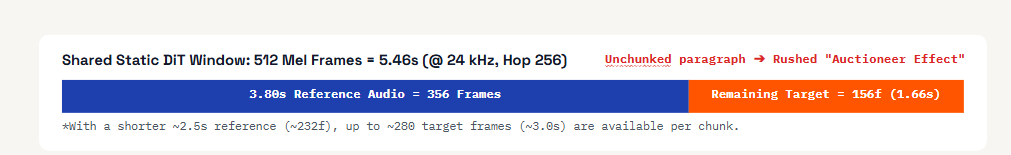
\includegraphics[width=\linewidth]{chunking-frame-budget.png}
\caption{Illustrative division of the fixed mel window between the
reference recording and target speech.}
\label{fig:chunk-budget}
\end{figure}

\texttt{MultilingualChunker.kt} protects decimal dots and common
abbreviations, then splits at sentence boundaries. It tries clause
boundaries and then word boundaries for oversized segments. It restores
protected punctuation and merges fragments shorter than 12 characters
when there is room. If it detects Devanagari, Tamil, Telugu or Kannada, it
uses a heuristic budget of 44 UTF-16 code units. The other inputs use 60.
These limits guide segmentation. The native runtime sets the final frame
allocation. For example, the input \emph{Open your books. Read the first
line.} becomes two ordered chunks, each consisting of one sentence.

\section{Extract and cache the reference mel}

After splitting the target text, the app calls \texttt{setReferenceAudio()}
once per job. \texttt{audio\_processor.cpp} measures the input RMS, raises
quiet non-negligible signals toward 0.1, applies reflection center padding
and windows each frame with a Hann window. It computes a 1,024-point FFT
every 256 samples, applies 100 mel filters and takes the log after applying
a small floor. \texttt{litert\_indic\_engine.cpp} caches the mel, reference
frame count and transcript for every chunk in the job.

\section{Allocate target duration and build model inputs}

Let $R$ be the cached reference frame count, $B_r$ the reference transcript
length in bytes and $B_g$ the target length in bytes. The inference engine
estimates a requested target length and limits it to the remaining window.
\[
G_0=\max\left(80,\left\lfloor
1.15 R\frac{\max(1,B_g)}{\max(1,B_r)}
\right\rfloor+10\right),\qquad G=\min(512-R,G_0).
\]
The requested 80-frame minimum applies before the cap. A long reference can
therefore leave fewer than 80 frames for target speech.

The engine copies the reference mel into the leading rows of a zero-filled
conditioning tensor. It combines the transcript and target chunk and
appends terminal punctuation when the native punctuation rule calls for
it. \texttt{indic\_tokenizer.cpp} maps the text to vocabulary IDs, truncates
or pads to 128 positions and uses $-1$ for padding and unknown entries.
The text-token limit applies independently of the acoustic window.

\section{Generate acoustic features with IndicF5}

\texttt{euler\_sampler.cpp} initializes the latent with Gaussian noise
and uses seed $42+$ the zero-based chunk index. Each step runs IndicF5 with
the reference mel and text, then runs the same graph with zero conditioning
and pad-only tokens. With $v_c$ and $v_u$ as the conditioned and
unconditioned predictions, the update is
\[
v=v_c+2.0(v_c-v_u),\qquad
x_{i+1}=\operatorname{clip}(x_i+(t_{i+1}-t_i)v,-4.5,4.5).
\]
For $N$ steps, the current cosine-sway coefficient of $-1$ gives
$t_i=1-\cos(\pi i/(2N))$. At the default 16 steps, each chunk makes 32
DiT invocations. The app reports chunk and sampling progress.
Cancellation is cooperative and takes effect when execution reaches a
sampling or chunk checkpoint.

\section{Reconstruct and join the waveform}

\texttt{litert\_indic\_engine.cpp} restores the reference mel prefix and
transposes the generated mel for Vocos. The decoder produces 513 complex
frequency bins per frame as real and imaginary planes.
\texttt{audio\_processor.cpp} performs the inverse transform with KissFFT,
overlaps Hann-windowed frames, normalizes by the window envelope and
removes center padding. The engine slices the region allocated to the
target after the reference section. When the cropped peak is at least
0.03, the engine scales it to 0.95.

\texttt{WaveformStitcher.kt} trims quiet edges with an amplitude threshold
of 0.012. It retains 25 ms at the leading and intermediate trailing edges
and 120 ms at the final trailing edge. It applies 5 ms raised-cosine fades,
inserts 30 ms of silence between chunks, appends 450 ms of trailing silence
and peak-normalizes the assembled waveform to 0.95. The app fades each
chunk individually and concatenates them in order.

\section{Save, play, download and share}

\texttt{GenerationHistoryManager.kt} writes one 24 kHz mono 16-bit PCM WAV
to app-private storage and updates the local clip library.
\texttt{AudioExporter.kt} uses MediaStore for Downloads on Android 10 and
later, with a legacy file path on earlier versions. The share action in
\texttt{MainActivity.kt} opens the Android share sheet with an
\texttt{audio/wav} content URI and temporary read access. The current
inference loop skips empty chunks. If some chunks succeed, a file can
therefore contain only part of the requested text.

\section{Worked example: trace one chunk to the WAV}
\label{sec:worked-example}

The first chunk in the two-sentence example is \emph{Open your books.}
It contains 16 ASCII bytes. For this trace, assume a 40-byte reference
transcript and 356 cached reference mel frames.

\begin{enumerate}[nosep]
  \item \textbf{Allocate the window.} The duration heuristic requests
        $\lfloor 1.15\times356\times16/40\rfloor+10=173$ target frames.
        The shared 512-frame window caps this at $512-356=156$ frames,
        a nominal target budget of about 1.66 seconds.
  \item \textbf{Prepare and sample.} The engine copies the reference mel into
        the first 356 rows of the conditioning tensor and encodes the
        transcript and target together. With seed 42 for chunk index zero,
        it takes 16 Euler steps. The conditioned and unconditioned passes
        make 32 IndicF5 calls in total.
  \item \textbf{Decode and crop.} One Vocos invocation decodes the sampled
        mel. After inverse reconstruction and center-padding removal, the
        512-frame output spans $511\times256=130{,}816$ samples. The native
        crop starts at $356\times256=91{,}136$ and ends at the available
        length, yielding 39,680 target samples (about 1.65 seconds) before
        stitching.
  \item \textbf{Join and save.} The stitcher trims and fades the chunk,
        inserts a 30 ms gap before the second chunk, and adds 450 ms of
        trailing silence after the last chunk. Kotlin writes one 24 kHz
        mono 16-bit PCM WAV. Its final duration depends on the retained
        samples from both chunks and the inserted silence.
\end{enumerate}

\chapter{Results, Validation and Conclusion}

\section{Archived device measurements}

The archived suite reports results on a Galaxy S23 with Snapdragon 8 Gen 2,
8 GB of RAM, Android 16 and five XNNPACK threads. The accompanying
presentation reports 16 steps. Build identifiers, exact prompts and
thermal logs for individual cases were unavailable. The suite includes
English, Hindi, Telugu and Tamil. Table~\ref{tab:measurements} summarizes the
cases, with RTF carried forward as reported. The tests used short, medium and paragraph prompts.

\begin{table}[htbp]
\centering
\caption{Archived Galaxy S23 results by language and prompt length}
\label{tab:measurements}
\small
\begin{tabular}{@{}llrrrr@{}}
\toprule
Prompt & Language & Audio (s) & Generation (s) & RTF & Peak RSS (MB) \\
\midrule
Short & English & 2.48 & 3.82 & 1.54 & 378 \\
Short & Hindi & 2.31 & 3.79 & 1.64 & 379 \\
Short & Telugu & 2.52 & 3.85 & 1.52 & 381 \\
Short & Tamil & 2.40 & 3.81 & 1.58 & 380 \\
\addlinespace
Medium & English & 7.12 & 10.84 & 1.52 & 384 \\
Medium & Hindi & 6.85 & 10.61 & 1.54 & 385 \\
Medium & Telugu & 7.30 & 11.02 & 1.50 & 386 \\
Medium & Tamil & 7.05 & 10.79 & 1.53 & 385 \\
\addlinespace
Paragraph & English & 15.82 & 23.85 & 1.50 & 387 \\
Paragraph & Hindi & 16.20 & 24.62 & 1.51 & 388 \\
Paragraph & Telugu & 15.65 & 23.78 & 1.51 & 389 \\
Paragraph & Tamil & 16.10 & 24.47 & 1.52 & 388 \\
\bottomrule
\end{tabular}
\end{table}

Across the 12 archived cases, RTF ranged from 1.50 to 1.64 and peak
resident memory from 378 to 389 MB. Later screenshots show RTF of 7.88
and 11.77 and displayed memory of 933 and 812 MB, respectively. These
screenshots show readings from saved clips with unknown build and device
conditions. They document separate runs with different measurement scope.

\section{Interpret current app telemetry}

Real-time factor (RTF) is compute time divided by output audio duration.
\texttt{MainActivity.kt} divides the sum of native chunk times by the
final stitched waveform duration. An RTF above one means generation took
longer than playback under that timing definition. Reference preparation,
Kotlin stitching and WAV writing fall outside the native chunk timer.
Full latency is the wall-clock interval from tapping Generate to save
completion.

\texttt{TelemetryMonitor.kt} reads \texttt{VmRSS} after stitching and before
saving. This reading is a point sample of resident memory. Peak RSS
requires sampling throughout the run. Model file size measures disk storage
and is reported separately.

\section{Tests and practical checks}

\texttt{MultilingualChunkerTest.kt} checks segmentation, punctuation and
abbreviations. \texttt{WaveformStitcherTest.kt} checks assembly, trimming
and normalization. Device verification should include a short sentence
and a paragraph in airplane mode after installation, followed by playback,
export and sharing. Listening to the resulting WAV can reveal missing
words and clipped endings.

To compare builds, record model hashes, device and Android version, input
audio and texts, sampling steps, threads and whether the run started cold.
Capture native timing, end-to-end time and peak memory separately. The
measurements in this report were carried forward from existing results.

\section{Conclusion and future work}

The project adapted pretrained IndicF5 and Vocos to a fixed-window LiteRT
deployment on Android. Chunking, cached reference features and waveform
stitching let the app generate paragraphs offline and save them as one
WAV. Future work should reproduce latency and peak memory on the latest
build, test acceleration and lower-step sampling, and evaluate naturalness,
intelligibility and speaker similarity.

\end{document}
